% ===================================================================
%  Week 3 — Spatial Filtering & Convolution
%  Compile: pdflatex -interaction=nonstopmode slides.tex  (twice)
% ===================================================================
\documentclass[10pt,aspectratio=169]{beamer}
% ===================================================================
%  Shared Beamer preamble for "Practical Image Processing"
%  English slides. Compile with pdfLaTeX.
% ===================================================================

\usetheme{metropolis}
\usepackage[T1]{fontenc}
\usepackage[utf8]{inputenc}
\usepackage{lmodern}
\usepackage{listings}
\usepackage{tcolorbox}
\usepackage{fontawesome5}
\usepackage{booktabs}
\usepackage{amsmath,amssymb}
\usepackage{tikz}
\usepackage{pgfplots}
\pgfplotsset{compat=1.17}
\usetikzlibrary{arrows.meta,positioning,shapes.geometric,fit,backgrounds,matrix}
\tcbuselibrary{skins,breakable}

% ---- Palette --------------------------------------------------------
\definecolor{coursePrimary}{HTML}{1B4965}   % deep blue
\definecolor{courseAccent}{HTML}{E76F51}    % coral
\definecolor{courseGood}{HTML}{2A9D8F}      % teal
\definecolor{courseBad}{HTML}{C0392B}       % red
\definecolor{courseInfo}{HTML}{2980B9}      % blue
\definecolor{codeBg}{HTML}{F5F6FA}
\definecolor{codeKw}{HTML}{8E44AD}
\definecolor{codeStr}{HTML}{2A9D8F}
\definecolor{codeCom}{HTML}{7F8C8D}

\setbeamercolor{frametitle}{bg=coursePrimary}
\setbeamercolor{progress bar}{fg=courseAccent}
\setbeamercolor{alerted text}{fg=courseAccent}
\metroset{block=fill,sectionpage=progressbar,numbering=fraction}

% ---- Code listings (Python is built into listings) -----------------
\lstdefinestyle{course}{
  backgroundcolor=\color{codeBg},
  basicstyle=\ttfamily\scriptsize,
  keywordstyle=\color{codeKw}\bfseries,
  stringstyle=\color{codeStr},
  commentstyle=\color{codeCom}\itshape,
  numberstyle=\tiny\color{codeCom},
  numbers=left, numbersep=6pt,
  showstringspaces=false, breaklines=true, breakatwhitespace=true,
  tabsize=4, columns=fullflexible,
  frame=single, framesep=4pt, rulecolor=\color{gray!30},
  keepspaces=true, upquote=true, language=Python,
}
\lstset{style=course}
\lstdefinelanguage{bash}{
  keywords={cd,pip,python,venv,source,import}, sensitive=true,
  morecomment=[l]{\#}, morestring=[b]', morestring=[b]",
}

% ---- Reusable callout boxes ----------------------------------------
\newtcolorbox{goodbox}[1][Good practice]{colback=courseGood!8,colframe=courseGood,
  fonttitle=\bfseries,title={\faCheck~#1},boxrule=0.6pt,left=4pt,right=4pt,top=3pt,bottom=3pt}
\newtcolorbox{badbox}[1][Pitfall]{colback=courseBad!8,colframe=courseBad,
  fonttitle=\bfseries,title={\faTimes~#1},boxrule=0.6pt,left=4pt,right=4pt,top=3pt,bottom=3pt}
\newtcolorbox{infobox}[1][Note]{colback=courseInfo!8,colframe=courseInfo,
  fonttitle=\bfseries,title={\faInfoCircle~#1},boxrule=0.6pt,left=4pt,right=4pt,top=3pt,bottom=3pt}
\newtcolorbox{mathbox}[1][Math]{colback=coursePrimary!6,colframe=coursePrimary,
  fonttitle=\bfseries,title={\faCalculator~#1},boxrule=0.6pt,left=4pt,right=4pt,top=3pt,bottom=3pt}

\newcommand{\keyidea}[1]{\begin{alertblock}{Key idea}#1\end{alertblock}}
\newcommand{\term}[1]{\textbf{\color{coursePrimary}#1}}
\newcommand{\code}[1]{\lstinline[basicstyle=\ttfamily\small]|#1|}

% ---- A helper to draw a small pixel grid, cells shaded by value ----
% \pixelgrid{ {10,20,120,200,240}, {30,60,130,180,230}, ... }
\newcommand{\pixelgrid}[1]{%
  \begin{tikzpicture}[font=\scriptsize,scale=0.6]
    \foreach \row [count=\ry] in {#1} {
      \foreach \val [count=\cx] in \row {
        \draw[gray,fill=coursePrimary!8] (\cx,-\ry) rectangle ++(1,-1);
        \node at (\cx+0.5,-\ry-0.5) {\val};
      }
    }
  \end{tikzpicture}}


\title{Spatial Filtering \& Convolution}
\subtitle{Week 3 — Operating on neighbourhoods}
\author{Practical Image Processing}
\date{Lecture 3 \textbullet\ 60--70 min}

\begin{document}

\maketitle

\begin{frame}{Recap \& today}
  \begin{columns}[T]
    \begin{column}{0.58\textwidth}
      \begin{itemize}
        \item Wk2: point ops look at one pixel. They can't blur, sharpen, or find edges.
        \item \alert{Today:} \term{spatial filters} — a small \term{kernel} slides over the
              image and combines each pixel with its \term{neighbours}. This is \term{convolution}.
      \end{itemize}
    \end{column}
    \begin{column}{0.42\textwidth}
      \begin{alertblock}{Why it matters}
        Smoothing removes noise; sharpening recovers detail; and convolution is the exact
        operation a CNN learns in Week 13.
      \end{alertblock}
    \end{column}
  \end{columns}
\end{frame}

\begin{frame}{Roadmap}\tableofcontents\end{frame}

% ==================================================================
\section{Convolution}
% ==================================================================

\begin{frame}{A kernel slides over the image}
  \begin{center}
  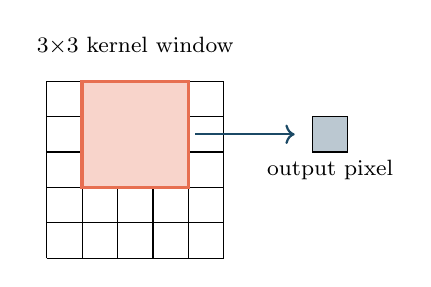
\begin{tikzpicture}[scale=0.45,font=\scriptsize]
    % image grid
    \foreach \x in {0,...,5} \draw (\x,0)--(\x,5);
    \foreach \y in {0,...,5} \draw (0,\y)--(5,\y);
    % 3x3 window highlighted
    \fill[courseAccent!30] (1,2) rectangle (4,5);
    \draw[courseAccent,very thick] (1,2) rectangle (4,5);
    \node at (2.5,6){\footnotesize 3$\times$3 kernel window};
    % output pixel
    \draw[->,coursePrimary,thick] (4.2,3.5)--(7,3.5);
    \fill[coursePrimary!30] (7.5,3) rectangle (8.5,4);
    \draw (7.5,3) rectangle (8.5,4);
    \node at (8,2.5){\footnotesize output pixel};
  \end{tikzpicture}
  \end{center}
  For each pixel: multiply the neighbourhood by the kernel, sum, write the result. Slide and repeat.
\end{frame}

\begin{frame}{Convolution, formally}
  \begin{mathbox}
    $g(x,y) = \displaystyle\sum_{i=-k}^{k}\sum_{j=-k}^{k} h(i,j)\, f(x-i,\,y-j)$
  \end{mathbox}
  \begin{itemize}
    \item $f$ = image, $h$ = kernel (a.k.a.\ filter/mask), $g$ = output.
    \item The kernel's values \emph{define} the operation: average $\rightarrow$ blur; differences $\rightarrow$ edges.
    \item Convolution flips the kernel; \term{correlation} doesn't. For symmetric kernels they're identical.
  \end{itemize}
\end{frame}

\begin{frame}{Two example kernels}
  \begin{columns}[T]
    \begin{column}{0.5\textwidth}
      \term{Box blur} (average):
      \[
      \frac{1}{9}\begin{bmatrix}1&1&1\\1&1&1\\1&1&1\end{bmatrix}
      \]
      Each output = mean of its 3$\times$3 neighbourhood.
    \end{column}
    \begin{column}{0.5\textwidth}
      \term{Sharpen}:
      \[
      \begin{bmatrix}0&-1&0\\-1&5&-1\\0&-1&0\end{bmatrix}
      \]
      Boosts the centre relative to its neighbours.
    \end{column}
  \end{columns}
  \vspace{4pt}
  \keyidea{The kernel \emph{is} the algorithm. Change the numbers, change the effect — nothing else.}
\end{frame}

\begin{frame}{Edge handling \& normalization}
  \begin{itemize}
    \item At the border the kernel hangs off the image — pad with zeros, replicate, or reflect (\code{borderType}).
    \item A blur kernel should \term{sum to 1} (preserve brightness); an edge kernel sums to 0.
    \item Kernel not normalized $\rightarrow$ the image gets darker/brighter as a side effect.
  \end{itemize}
  \begin{badbox}
    Forgetting to normalize a blur kernel is why a ``smoothed'' image sometimes comes out too dark.
  \end{badbox}
\end{frame}

% ==================================================================
\section{Smoothing}
% ==================================================================

\begin{frame}{Box vs Gaussian blur — on a real plate}
  \begin{columns}[T]
    \begin{column}{0.33\textwidth}\begin{center}
      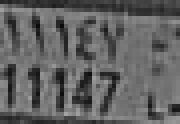
\includegraphics[width=\linewidth]{../assets/plate_gray.png}\\{\scriptsize original}
    \end{center}\end{column}
    \begin{column}{0.33\textwidth}\begin{center}
      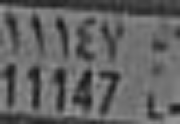
\includegraphics[width=\linewidth]{../assets/plate_box.png}\\{\scriptsize box blur 5$\times$5}
    \end{center}\end{column}
    \begin{column}{0.33\textwidth}\begin{center}
      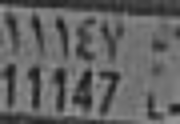
\includegraphics[width=\linewidth]{../assets/plate_gauss.png}\\{\scriptsize Gaussian $\sigma$=1.5}
    \end{center}\end{column}
  \end{columns}
  \vspace{3pt}
  Box averages equally (boxy artifacts); Gaussian weights the centre more (smoother, natural).
\end{frame}

\begin{frame}{The Gaussian kernel}
  \begin{mathbox}
    $h(i,j) = \dfrac{1}{2\pi\sigma^2}\,e^{-(i^2+j^2)/(2\sigma^2)}$
  \end{mathbox}
  \begin{itemize}
    \item \term{$\sigma$} controls the blur amount; larger $\sigma$ = more smoothing, wider kernel.
    \item \term{Separable}: a 2D Gaussian = a 1D horizontal blur then a 1D vertical blur $\rightarrow$ much faster.
    \item The go-to smoother: removes noise while preserving structure better than a box.
  \end{itemize}
\end{frame}

\begin{frame}{Why smooth at all?}
  \begin{itemize}
    \item Remove noise before thresholding/edges (noise creates false edges — Week 5).
    \item Blur \emph{before} downsampling to avoid aliasing (Week 1's Nyquist).
    \item Suppress fine texture so large structures dominate (find the page, not the paper grain).
  \end{itemize}
  \begin{badbox}
    But blur also destroys detail. Too much and the digits smear together — a trade-off you tune.
  \end{badbox}
\end{frame}

% ==================================================================
\section{Sharpening}
% ==================================================================

\begin{frame}{Sharpening = add back the detail}
  \begin{columns}[T]
    \begin{column}{0.5\textwidth}\begin{center}
      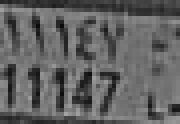
\includegraphics[width=0.9\linewidth]{../assets/plate_gray.png}\\{\scriptsize original}\\[4pt]
      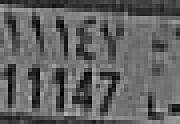
\includegraphics[width=0.9\linewidth]{../assets/plate_sharp.png}\\{\scriptsize unsharp-masked}
    \end{center}\end{column}
    \begin{column}{0.5\textwidth}
      \begin{itemize}
        \item \term{Unsharp mask}: $\text{sharp} = \text{img} + \lambda(\text{img}-\text{blur})$.
        \item The $(\text{img}-\text{blur})$ term \emph{is} the high-frequency detail.
        \item Adds it back to emphasize edges — the digits' strokes stand out.
      \end{itemize}
    \end{column}
  \end{columns}
\end{frame}

\begin{frame}{Sharpening's catch}
  \begin{itemize}
    \item It amplifies \emph{everything} high-frequency — including noise and JPEG blocks.
    \item Over-sharpening creates \term{halos} (bright/dark rings) around edges.
    \item Denoise first, then sharpen gently. Never sharpen a noisy image blindly.
  \end{itemize}
  \keyidea{Blur and sharpen are opposites, but they're both convolution — just different kernels.}
\end{frame}

\begin{frame}{A zoo of kernels}
  \begin{center}
  \begin{tabular}{@{}ll@{}}
    \toprule
    \textbf{Kernel} & \textbf{Effect} \\
    \midrule
    all $1/n$ & box blur (average) \\
    Gaussian weights & smooth blur \\
    centre 5, sides $-1$ & sharpen (high-pass) \\
    $[-1,0,1]$ rows & horizontal gradient (edges, Week 5) \\
    identity + (id $-$ blur) & unsharp mask \\
    \bottomrule
  \end{tabular}
  \end{center}
  \keyidea{You don't memorize kernels — you understand what ``average'' vs ``difference'' does, and design the rest.}
\end{frame}

\begin{frame}{Bilateral filter: smooth but keep edges}
  \begin{itemize}
    \item Gaussian blur smears edges; the \term{bilateral} filter weights by \emph{both} distance \emph{and} intensity similarity.
    \item Result: flat regions get smoothed, edges stay crisp — great before thresholding a document.
    \item Slower, but often the right smoother for DocScan: \code{cv2.bilateralFilter}.
  \end{itemize}
  \begin{goodbox}
    When you need to denoise \emph{without} blurring the digit edges, reach for bilateral (or median).
  \end{goodbox}
\end{frame}

% ==================================================================
\section{In-class exercise}
% ==================================================================

\begin{frame}[fragile]{\faPen~In-class exercise (12 min)}
  \begin{infobox}[Convolve by hand]
  \end{infobox}
  A 3$\times$3 patch and a kernel:
  \[
  P=\begin{bmatrix}10&10&10\\10&50&10\\10&10&10\end{bmatrix}\qquad
  K=\begin{bmatrix}0&-1&0\\-1&5&-1\\0&-1&0\end{bmatrix}
  \]
  \begin{enumerate}
    \item Compute the output for the centre pixel (element-wise multiply, then sum).
    \item What does this kernel do to the centre value? What kind of filter is it?
    \item Now use the box-blur kernel instead. What is the centre output?
  \end{enumerate}
\end{frame}

\begin{frame}{\faPen~Debrief}
  \begin{itemize}
    \item Sharpen: $5(50) - 10 - 10 - 10 - 10 = 250 - 40 = 210$. The centre (50) jumped to 210 — \emph{contrast boosted}.
    \item It's a \term{high-pass} filter: it emphasizes the difference between centre and surround.
    \item Box blur: $(10{\cdot}8 + 50)/9 = 130/9 \approx 14$. The bright centre was \emph{averaged down} — smoothed.
  \end{itemize}
  \keyidea{Same patch, two kernels, opposite effects. The kernel is everything.}
\end{frame}

% ==================================================================
\section{Deep dive}
% ==================================================================

\begin{frame}{Frequency view: low-pass vs high-pass}
  \begin{itemize}
    \item Smoothing keeps \term{low frequencies} (slow changes), removes high (a \term{low-pass} filter).
    \item Sharpening/edges keep \term{high frequencies} (fast changes) — a \term{high-pass} filter.
    \item Week 6 makes this literal with the Fourier transform; today it's intuition.
  \end{itemize}
  \begin{goodbox}
    ``Blur = low-pass, edges = high-pass'' is a lens you'll use for the rest of the course.
  \end{goodbox}
\end{frame}

\begin{frame}{Separability \& speed}
  \begin{itemize}
    \item A separable 2D kernel = outer product of two 1D kernels; apply them in sequence.
    \item A $k\times k$ blur costs $k^2$ multiplies per pixel; separated, only $2k$ — a big win for large $k$.
    \item OpenCV does this automatically for Gaussian; know it so you write fast filters.
  \end{itemize}
\end{frame}

\begin{frame}{Nonlinear filter preview: median}
  \begin{columns}[T]
    \begin{column}{0.5\textwidth}\begin{center}
      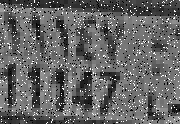
\includegraphics[width=0.85\linewidth]{../assets/plate_noisy.png}\\{\scriptsize salt-and-pepper noise}\\[3pt]
      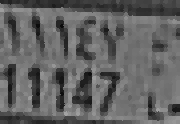
\includegraphics[width=0.85\linewidth]{../assets/plate_median.png}\\{\scriptsize 3$\times$3 median}
    \end{center}\end{column}
    \begin{column}{0.5\textwidth}
      \begin{itemize}
        \item A \term{median} filter takes the median of the neighbourhood — not a weighted sum.
        \item It kills salt-and-pepper noise while keeping edges sharp (a Gaussian would smear them).
        \item Nonlinear $\rightarrow$ not convolution, but same ``slide a window'' idea. Full story in Week 4.
      \end{itemize}
    \end{column}
  \end{columns}
\end{frame}

\begin{frame}{Convolution is the bridge to deep learning}
  \begin{itemize}
    \item A CNN layer (Week 13) is exactly this: convolve the image with small kernels.
    \item The difference: the network \emph{learns} the kernel values from data instead of you designing them.
    \item Everything you learn about kernels today is what a CNN's first layers do.
  \end{itemize}
  \keyidea{Classical filters are hand-designed kernels; CNNs are learned kernels. Same operation.}
\end{frame}

\begin{frame}[fragile]{Filtering in code}
\begin{lstlisting}[language=Python]
box    = cv2.blur(img, (5, 5))
gauss  = cv2.GaussianBlur(img, (7, 7), 1.5)
median = cv2.medianBlur(img, 3)
k = np.array([[0,-1,0],[-1,5,-1],[0,-1,0]])
sharp  = cv2.filter2D(img, -1, k)          # apply any custom kernel
\end{lstlisting}
  \code{cv2.filter2D} convolves with any kernel you give it — the general tool.
\end{frame}

% ==================================================================
\section{Wrap-up}
% ==================================================================

\begin{frame}{What you should now be able to do}
  \begin{itemize}
    \item Explain convolution and how a kernel defines an operation.
    \item Smooth with box/Gaussian; sharpen with unsharp mask; know the trade-offs.
    \item Handle borders and normalization; exploit separability for speed.
    \item See the low-pass/high-pass view and the link to CNNs.
  \end{itemize}
\end{frame}

\begin{frame}{This week's deliverable}
  \begin{alertblock}{Due before Week 4 (see \code{project/})}
    On real meter/plate images:
    \begin{enumerate}
      \item Implement a 3$\times$3 convolution \emph{from scratch} (NumPy) and match \code{cv2.filter2D}.
      \item Compare box vs Gaussian blur at several sizes; discuss detail loss vs noise removal.
      \item Sharpen a plate with unsharp mask; find where it starts creating halos.
      \item Note: what blur helps your DocScan threshold, and what over-blurs the digits?
    \end{enumerate}
  \end{alertblock}
\end{frame}

\begin{frame}[standout]
  The kernel is the algorithm.\\[4pt]
  \normalsize Blur, sharpen, edges — all the same operation with different numbers.
\end{frame}

\end{document}
